\documentclass[border=5]{standalone}
\usepackage{calculator}
\usepackage{tikz}
\usetikzlibrary{arrows, arrows.meta, positioning}

\tikzset{    
    disk/.style={ thick },
    traj/.style={ thin, dashed, -Latex },
    point/.style={ color=black, circle, scale=0.3, fill },
    partition/.style={ right, scale=0.75 },
    label/.style={ scale=0.5, black, below = 0.5mm },
    time/.style={ scale=0.75, above left }
}

\definecolor{light-gray}{gray}{0.45}

\def\xMin{0}
\def\xMax{2}
\def\yMin{0}
\def\yMax{2}
\def\xWidth{2}
\def\oPacity{0.75}
\def\ySlant{0.5}
\def\xSlant{-0.9}
\def\z{6.75}
\def\speed{0.2}
\def\R{0.075}

\newcommand{\drawBlueFrame}[5]{
    \fill[blue, opacity=0.05] (#1*\xWidth-#5,#2*\xWidth-#5) rectangle (#3*\xWidth+#5,#4*\xWidth+#5);
    \draw[blue, opacity=0.05] (#1*\xWidth-#5,#2*\xWidth-#5) rectangle (#3*\xWidth+#5,#4*\xWidth+#5);
}

\newcommand{\drawWhiteFrameB}[5]{
    \fill[white, opacity=0.5] (#1*\xWidth-#5,#2*\xWidth-#5) rectangle (#3*\xWidth+#5,#4*\xWidth+#5);
    \draw[black, dashed, opacity=0.5] (#1*\xWidth-#5,#2*\xWidth-#5) rectangle (#3*\xWidth+#5,#4*\xWidth+#5);
}

\newcommand{\drawGrid}{
    \fill[white,fill opacity=\oPacity] (\xMin,\yMin) rectangle (\xMax,\yMax);
    \draw[step=\xWidth, very thin, light-gray] (\xMin,\yMin) grid (\xMax,\yMax);
}
\newcommand{\drawFlocks}[1]{
    \draw [fill=lime]   (A#1) circle (\R) ;
    \draw [fill=magenta](B#1) circle (\R) ;
    \draw [fill=teal]   (C#1) circle (\R) ;
    \draw [fill=olive]  (D#1) circle (\R) ;
}
\newcommand{\drawLabels}[1]{
    \node[label] at (A#1) {$a$};
    \node[label] at (B#1) {$b$};
    \node[label] at (C#1) {$c$};
    \node[label] at (D#1) {$d$};
}
\newcommand{\drawTrajs}[2]{
        \draw[traj] (A#1) -- (A#2);
        \draw[traj] (B#1) -- (B#2);
        \draw[traj] (C#1) -- (C#2);
        \draw[traj] (D#1) -- (D#2);
}

\begin{document}
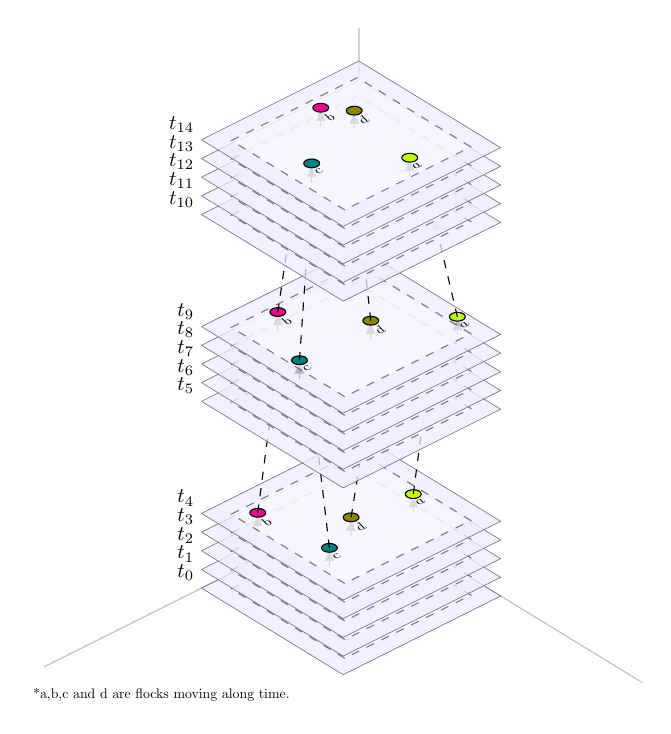
\begin{tikzpicture}    
    \def\t{0};
    \begin{scope}
        [yshift=0*\z, every node/.append style={yslant=\ySlant,xslant=\xSlant},yslant=\ySlant,xslant=\xSlant]
        \coordinate (T) at (\xMin, \xMax);
        \coordinate (O) at (\xMax,\yMax);

        \draw[black!25] (O) -- (\xMax,-2);
        \draw[black!25] (O) -- (-2,\yMax);
        \draw[black!25] (O) -- (7.5,8.11);
        \drawGrid
        \drawBlueFrame{0}{0}{1}{1}{\t*\speed};
        \drawWhiteFrameB{0}{0}{1}{1}{-1*\speed};
    \end{scope}
    \node[time] at (T) {$t_\t$};
    \draw[] (-4.0,-0.25) node[scale=0.5,right]{*a,b,c and d are flocks moving along time.};

    \def\t{1};
    \begin{scope}
        [yshift=1*\z, every node/.append style={yslant=\ySlant,xslant=\xSlant},yslant=\ySlant,xslant=\xSlant]
        \coordinate (T) at (\xMin, \xMax);

        \drawGrid
        \drawBlueFrame{0}{0}{1}{1}{0*\speed};
        \drawWhiteFrameB{0}{0}{1}{1}{-1*\speed};
    \end{scope}
    \node[time] at (T) {$t_\t$};
    
    \def\t{2};
    \begin{scope}
        [yshift=2*\z, every node/.append style={yslant=\ySlant,xslant=\xSlant},yslant=\ySlant,xslant=\xSlant]
        \coordinate (T) at (\xMin, \xMax);

        \drawGrid
        \drawBlueFrame{0}{0}{1}{1}{0*\speed};
        \drawWhiteFrameB{0}{0}{1}{1}{-1*\speed};
    \end{scope}
    \node[time] at (T) {$t_\t$};

    \def\t{3};
    \begin{scope}
        [yshift=3*\z, every node/.append style={yslant=\ySlant,xslant=\xSlant},yslant=\ySlant,xslant=\xSlant]
        \coordinate (T) at (\xMin, \xMax);
        \coordinate (A\t) at (1.70, 0.90);
        \coordinate (B\t) at (0.40, 1.65);
        \coordinate (C\t) at (0.50, 0.75);
        \coordinate (D\t) at (1.00, 1.00);

        \drawGrid
        \drawBlueFrame{0}{0}{1}{1}{0*\speed};
        \drawWhiteFrameB{0}{0}{1}{1}{-1*\speed};
    \end{scope}
    \node[time] at (T) {$t_\t$};
    
    \def\t{4};
    \begin{scope}
        [yshift=4*\z, every node/.append style={yslant=\ySlant,xslant=\xSlant},yslant=\ySlant,xslant=\xSlant]
        \coordinate (T) at (\xMin, \xMax);
        \coordinate (A\t) at (1.70, 0.90);
        \coordinate (B\t) at (0.40, 1.65);
        \coordinate (C\t) at (0.50, 0.75);
        \coordinate (D\t) at (1.00, 1.00);

        \drawTrajs{3}{4}
        \drawGrid
        \drawBlueFrame{0}{0}{1}{1}{0*\speed};
        \drawWhiteFrameB{0}{0}{1}{1}{-1*\speed};
        \drawFlocks{4}
        \drawLabels{4}

    \end{scope}
    \node[time] at (T) {$t_\t$};

    %%%%%%%

    \def\t{10};
    \begin{scope}
        [yshift=\t*\z, every node/.append style={yslant=\ySlant,xslant=\xSlant},yslant=\ySlant,xslant=\xSlant]
        \coordinate (T) at (\xMin, \xMax);
        \coordinate (A\t) at (1.90, 0.90);
        \coordinate (B\t) at (0.60, 1.65);
        \coordinate (C\t) at (0.50, 0.95);
        \coordinate (D\t) at (1.25, 1.00);

        \drawTrajs{4}{10}
        \drawGrid
        \drawBlueFrame{0}{0}{1}{1}{0*\speed};
        \drawWhiteFrameB{0}{0}{1}{1}{-1*\speed};
    \end{scope}
    \node[time] at (T) {$t_{5}$};

    \def\t{11};
    \begin{scope}
        [yshift=\t*\z, every node/.append style={yslant=\ySlant,xslant=\xSlant},yslant=\ySlant,xslant=\xSlant]
        \coordinate (T) at (\xMin, \xMax);
        \drawGrid
        \drawBlueFrame{0}{0}{1}{1}{0*\speed};
        \drawWhiteFrameB{0}{0}{1}{1}{-1*\speed};
        %\drawFlocks{10}
        %\drawLabels{0}
    \end{scope}
    \node[time] at (T) {$t_{6}$};
    \def\t{12};
    \begin{scope}
        [yshift=\t*\z, every node/.append style={yslant=\ySlant,xslant=\xSlant},yslant=\ySlant,xslant=\xSlant]
        \coordinate (T) at (\xMin, \xMax);
        \drawGrid
        \drawBlueFrame{0}{0}{1}{1}{0*\speed};
        \drawWhiteFrameB{0}{0}{1}{1}{-1*\speed};
    \end{scope}
    \node[time] at (T) {$t_{7}$};
    \def\t{13};
    \begin{scope}
        [yshift=\t*\z, every node/.append style={yslant=\ySlant,xslant=\xSlant},yslant=\ySlant,xslant=\xSlant]
        \coordinate (T) at (\xMin, \xMax);
        \coordinate (A\t) at (1.90, 0.50);
        \coordinate (B\t) at (0.70, 1.70);
        \coordinate (C\t) at (0.30, 0.95);
        \coordinate (D\t) at (1.25, 1.00);

        \drawGrid
        \drawBlueFrame{0}{0}{1}{1}{0*\speed};
        \drawWhiteFrameB{0}{0}{1}{1}{-1*\speed};
    \end{scope}
    \node[time] at (T) {$t_{8}$};
    \def\t{14};
    \begin{scope}
        [yshift=\t*\z, every node/.append style={yslant=\ySlant,xslant=\xSlant},yslant=\ySlant,xslant=\xSlant]
        \coordinate (T) at (\xMin, \xMax);
        \coordinate (A\t) at (1.90, 0.50);
        \coordinate (B\t) at (0.70, 1.70);
        \coordinate (C\t) at (0.30, 0.95);
        \coordinate (D\t) at (1.25, 1.00);

        \drawTrajs{13}{14}
        \drawGrid
        \drawBlueFrame{0}{0}{1}{1}{0*\speed};
        \drawWhiteFrameB{0}{0}{1}{1}{-1*\speed};
        \drawFlocks{14}
        \drawLabels{14}
    \end{scope}
    \node[time] at (T) {$t_{9}$};

    %%%%%%%

    \def\t{20};
    \begin{scope}
        [yshift=\t*\z, every node/.append style={yslant=\ySlant,xslant=\xSlant},yslant=\ySlant,xslant=\xSlant]
        \coordinate (T) at (\xMin, \xMax);
        \coordinate (A\t) at (1.60, 0.50);
        \coordinate (B\t) at (1.40, 2.15);
        \coordinate (C\t) at (0.50, 1.05);
        \coordinate (D\t) at (1.50, 1.50);

        \drawTrajs{14}{20}
        \drawGrid
        \drawBlueFrame{0}{0}{1}{1}{0*\speed};
        \drawWhiteFrameB{0}{0}{1}{1}{-1*\speed};
    \end{scope}
    \node[time] at (T) {$t_{10}$};
    \def\t{21};
    \begin{scope}
        [yshift=\t*\z, every node/.append style={yslant=\ySlant,xslant=\xSlant},yslant=\ySlant,xslant=\xSlant]
        \coordinate (T) at (\xMin, \xMax);
        \drawGrid
        \drawBlueFrame{0}{0}{1}{1}{0*\speed};
        \drawWhiteFrameB{0}{0}{1}{1}{-1*\speed};
    \end{scope}
    \node[time] at (T) {$t_{11}$};
    \def\t{22};
    \begin{scope}
        [yshift=\t*\z, every node/.append style={yslant=\ySlant,xslant=\xSlant},yslant=\ySlant,xslant=\xSlant]
        \coordinate (T) at (\xMin, \xMax);
        \drawGrid
        \drawBlueFrame{0}{0}{1}{1}{0*\speed};
        \drawWhiteFrameB{0}{0}{1}{1}{-1*\speed};
    \end{scope}
    \node[time] at (T) {$t_{12}$};
    \def\t{23};
    \begin{scope}
        [yshift=\t*\z, every node/.append style={yslant=\ySlant,xslant=\xSlant},yslant=\ySlant,xslant=\xSlant]
        \coordinate (T) at (\xMin, \xMax);
        \coordinate (A\t) at (1.25, 0.45);
        \coordinate (B\t) at (1.20, 1.65);
        \coordinate (C\t) at (0.50, 1.00);
        \coordinate (D\t) at (1.40, 1.40);

        \drawGrid
        \drawBlueFrame{0}{0}{1}{1}{0*\speed};
        \drawWhiteFrameB{0}{0}{1}{1}{-1*\speed};
    \end{scope}
    \node[time] at (T) {$t_{13}$};
    \def\t{24};
    \begin{scope}
        [yshift=\t*\z, every node/.append style={yslant=\ySlant,xslant=\xSlant},yslant=\ySlant,xslant=\xSlant]
        \coordinate (T) at (\xMin, \xMax);
        \coordinate (A\t) at (1.25, 0.45);
        \coordinate (B\t) at (1.20, 1.65);
        \coordinate (C\t) at (0.50, 1.00);
        \coordinate (D\t) at (1.40, 1.40);

        \drawTrajs{23}{24}
        \drawGrid
        \drawBlueFrame{0}{0}{1}{1}{0*\speed};
        \drawWhiteFrameB{0}{0}{1}{1}{-1*\speed};
        \drawFlocks{24}
        \drawLabels{24}
    \end{scope}
    \node[time] at (T) {$t_{14}$};

\end{tikzpicture}
\end{document} 
